\subsection{Breadth-first search}

\emph{Breadth-first search}, or \emph{BFS} uses a queue as a waiting list,
and that is literally the only difference in the implementation.

What changes is the order the nodes will be processed in.
Since the nodes are taken from the queue
in the same order as they were inserted,
the algorithm will first process all the neighbours of the starting point,
then when it has done that it will process the neighbours of the neighbours,
etc. It will work its way \emph{by layers}.

The diagram below shows the order in which nodes are visited for
the same example:
\begin{center}
    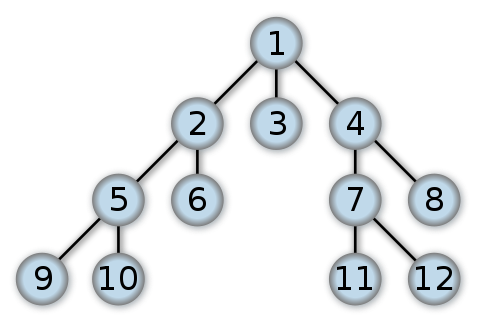
\includegraphics[width=0.3\textwidth]{img/bfs}
\end{center}

The advantage of BFS is that if we keep track of which edges it took
to get to the nodes, it gives us the shortest path from the starting point
to every node.
That is because of the order in which BFS visits the nodes.
It first makes sure all the nodes at distance 1 have been processed before
moving on to the nodes at distance 2, so we can be sure there was no path
shorter than 2. The same applies for distance 3, then 4, and so on.

Note that it only gives the shortest path in terms of number of edges.
If the edges have different costs (that is, if the graph is weighted),
then BFS will not work.
